\documentclass[]{article}
\usepackage{lmodern}
\usepackage{amssymb,amsmath}
\usepackage{ifxetex,ifluatex}
\usepackage{fixltx2e} % provides \textsubscript
\ifnum 0\ifxetex 1\fi\ifluatex 1\fi=0 % if pdftex
  \usepackage[T1]{fontenc}
  \usepackage[utf8]{inputenc}
\else % if luatex or xelatex
  \ifxetex
    \usepackage{mathspec}
  \else
    \usepackage{fontspec}
  \fi
  \defaultfontfeatures{Ligatures=TeX,Scale=MatchLowercase}
\fi
% use upquote if available, for straight quotes in verbatim environments
\IfFileExists{upquote.sty}{\usepackage{upquote}}{}
% use microtype if available
\IfFileExists{microtype.sty}{%
\usepackage{microtype}
\UseMicrotypeSet[protrusion]{basicmath} % disable protrusion for tt fonts
}{}
\usepackage[margin=1in]{geometry}
\usepackage{hyperref}
\hypersetup{unicode=true,
            pdfborder={0 0 0},
            breaklinks=true}
\urlstyle{same}  % don't use monospace font for urls
\usepackage{color}
\usepackage{fancyvrb}
\newcommand{\VerbBar}{|}
\newcommand{\VERB}{\Verb[commandchars=\\\{\}]}
\DefineVerbatimEnvironment{Highlighting}{Verbatim}{commandchars=\\\{\}}
% Add ',fontsize=\small' for more characters per line
\usepackage{framed}
\definecolor{shadecolor}{RGB}{248,248,248}
\newenvironment{Shaded}{\begin{snugshade}}{\end{snugshade}}
\newcommand{\KeywordTok}[1]{\textcolor[rgb]{0.13,0.29,0.53}{\textbf{#1}}}
\newcommand{\DataTypeTok}[1]{\textcolor[rgb]{0.13,0.29,0.53}{#1}}
\newcommand{\DecValTok}[1]{\textcolor[rgb]{0.00,0.00,0.81}{#1}}
\newcommand{\BaseNTok}[1]{\textcolor[rgb]{0.00,0.00,0.81}{#1}}
\newcommand{\FloatTok}[1]{\textcolor[rgb]{0.00,0.00,0.81}{#1}}
\newcommand{\ConstantTok}[1]{\textcolor[rgb]{0.00,0.00,0.00}{#1}}
\newcommand{\CharTok}[1]{\textcolor[rgb]{0.31,0.60,0.02}{#1}}
\newcommand{\SpecialCharTok}[1]{\textcolor[rgb]{0.00,0.00,0.00}{#1}}
\newcommand{\StringTok}[1]{\textcolor[rgb]{0.31,0.60,0.02}{#1}}
\newcommand{\VerbatimStringTok}[1]{\textcolor[rgb]{0.31,0.60,0.02}{#1}}
\newcommand{\SpecialStringTok}[1]{\textcolor[rgb]{0.31,0.60,0.02}{#1}}
\newcommand{\ImportTok}[1]{#1}
\newcommand{\CommentTok}[1]{\textcolor[rgb]{0.56,0.35,0.01}{\textit{#1}}}
\newcommand{\DocumentationTok}[1]{\textcolor[rgb]{0.56,0.35,0.01}{\textbf{\textit{#1}}}}
\newcommand{\AnnotationTok}[1]{\textcolor[rgb]{0.56,0.35,0.01}{\textbf{\textit{#1}}}}
\newcommand{\CommentVarTok}[1]{\textcolor[rgb]{0.56,0.35,0.01}{\textbf{\textit{#1}}}}
\newcommand{\OtherTok}[1]{\textcolor[rgb]{0.56,0.35,0.01}{#1}}
\newcommand{\FunctionTok}[1]{\textcolor[rgb]{0.00,0.00,0.00}{#1}}
\newcommand{\VariableTok}[1]{\textcolor[rgb]{0.00,0.00,0.00}{#1}}
\newcommand{\ControlFlowTok}[1]{\textcolor[rgb]{0.13,0.29,0.53}{\textbf{#1}}}
\newcommand{\OperatorTok}[1]{\textcolor[rgb]{0.81,0.36,0.00}{\textbf{#1}}}
\newcommand{\BuiltInTok}[1]{#1}
\newcommand{\ExtensionTok}[1]{#1}
\newcommand{\PreprocessorTok}[1]{\textcolor[rgb]{0.56,0.35,0.01}{\textit{#1}}}
\newcommand{\AttributeTok}[1]{\textcolor[rgb]{0.77,0.63,0.00}{#1}}
\newcommand{\RegionMarkerTok}[1]{#1}
\newcommand{\InformationTok}[1]{\textcolor[rgb]{0.56,0.35,0.01}{\textbf{\textit{#1}}}}
\newcommand{\WarningTok}[1]{\textcolor[rgb]{0.56,0.35,0.01}{\textbf{\textit{#1}}}}
\newcommand{\AlertTok}[1]{\textcolor[rgb]{0.94,0.16,0.16}{#1}}
\newcommand{\ErrorTok}[1]{\textcolor[rgb]{0.64,0.00,0.00}{\textbf{#1}}}
\newcommand{\NormalTok}[1]{#1}
\usepackage{graphicx,grffile}
\makeatletter
\def\maxwidth{\ifdim\Gin@nat@width>\linewidth\linewidth\else\Gin@nat@width\fi}
\def\maxheight{\ifdim\Gin@nat@height>\textheight\textheight\else\Gin@nat@height\fi}
\makeatother
% Scale images if necessary, so that they will not overflow the page
% margins by default, and it is still possible to overwrite the defaults
% using explicit options in \includegraphics[width, height, ...]{}
\setkeys{Gin}{width=\maxwidth,height=\maxheight,keepaspectratio}
\IfFileExists{parskip.sty}{%
\usepackage{parskip}
}{% else
\setlength{\parindent}{0pt}
\setlength{\parskip}{6pt plus 2pt minus 1pt}
}
\setlength{\emergencystretch}{3em}  % prevent overfull lines
\providecommand{\tightlist}{%
  \setlength{\itemsep}{0pt}\setlength{\parskip}{0pt}}
\setcounter{secnumdepth}{0}
% Redefines (sub)paragraphs to behave more like sections
\ifx\paragraph\undefined\else
\let\oldparagraph\paragraph
\renewcommand{\paragraph}[1]{\oldparagraph{#1}\mbox{}}
\fi
\ifx\subparagraph\undefined\else
\let\oldsubparagraph\subparagraph
\renewcommand{\subparagraph}[1]{\oldsubparagraph{#1}\mbox{}}
\fi

%%% Use protect on footnotes to avoid problems with footnotes in titles
\let\rmarkdownfootnote\footnote%
\def\footnote{\protect\rmarkdownfootnote}

%%% Change title format to be more compact
\usepackage{titling}

% Create subtitle command for use in maketitle
\newcommand{\subtitle}[1]{
  \posttitle{
    \begin{center}\large#1\end{center}
    }
}

\setlength{\droptitle}{-2em}

  \title{2018R1 High-Dimensional Data Analysis (STAT5103) Assignment 3}
    \pretitle{\vspace{\droptitle}\centering\huge}
  \posttitle{\par}
    \author{Yiu Chung WONG 1155017920}
    \preauthor{\centering\large\emph}
  \postauthor{\par}
    \date{}
    \predate{}\postdate{}
  

\begin{document}
\maketitle

\section{Principal Component Analysis (PCA) on carm Car
Dataset}\label{principal-component-analysis-pca-on-carm-car-dataset}

\begin{Shaded}
\begin{Highlighting}[]
\NormalTok{pc_car <-}\StringTok{ }\KeywordTok{read.csv}\NormalTok{(}\StringTok{'carm.txt'}\NormalTok{, }\DataTypeTok{header =} \OtherTok{FALSE}\NormalTok{, }\DataTypeTok{sep =} \StringTok{''}\NormalTok{)}
\NormalTok{names <-}\StringTok{ }\KeywordTok{c}\NormalTok{(}\StringTok{"Model"}\NormalTok{, }\StringTok{"Economy"}\NormalTok{, }\StringTok{"Service"}\NormalTok{, }\StringTok{"Non-depreciation_of_value"}\NormalTok{, }\StringTok{"Price"}\NormalTok{, }\StringTok{"Design"}\NormalTok{, }\StringTok{"Sporty_car"}\NormalTok{, }\StringTok{"Safety"}\NormalTok{, }\StringTok{"Easy_handling"}\NormalTok{)}
\KeywordTok{names}\NormalTok{(pc_car) <-}\StringTok{ }\NormalTok{names}
\KeywordTok{rownames}\NormalTok{(pc_car) <-}\StringTok{ }\NormalTok{pc_car[,}\DecValTok{1}\NormalTok{]}
\NormalTok{pc_car <-}\StringTok{ }\NormalTok{pc_car[,}\OperatorTok{-}\DecValTok{1}\NormalTok{]}
\KeywordTok{summary}\NormalTok{(pc_car)}
\end{Highlighting}
\end{Shaded}

\begin{verbatim}
##     Economy         Service      Non-depreciation_of_value     Price           Design   
##  Min.   :2.100   Min.   :1.600   Min.   :1.600             Min.   :1.500   Min.   :1.3  
##  1st Qu.:2.600   1st Qu.:2.500   1st Qu.:2.200             1st Qu.:2.600   1st Qu.:2.9  
##  Median :3.100   Median :2.900   Median :3.200             Median :3.000   Median :3.2  
##  Mean   :3.291   Mean   :3.061   Mean   :3.152             Mean   :3.274   Mean   :3.2  
##  3rd Qu.:3.850   3rd Qu.:3.450   3rd Qu.:3.750             3rd Qu.:4.100   3rd Qu.:3.6  
##  Max.   :5.300   Max.   :4.700   Max.   :5.500             Max.   :5.900   Max.   :4.8  
##    Sporty_car        Safety      Easy_handling  
##  Min.   :1.100   Min.   :1.400   Min.   :1.800  
##  1st Qu.:3.050   1st Qu.:2.800   1st Qu.:2.400  
##  Median :3.300   Median :3.200   Median :2.700  
##  Mean   :3.465   Mean   :3.287   Mean   :2.787  
##  3rd Qu.:3.950   3rd Qu.:3.750   3rd Qu.:2.950  
##  Max.   :5.800   Max.   :5.900   Max.   :4.300
\end{verbatim}

\section{Analyzing carm.txt dataset}\label{analyzing-carm.txt-dataset}

carm.txt data sets comes with basic dataset with 8 variables. Using PCA,
we are going to find linear combinations of the variables that both
maximises variance and are mutually uncorrelated.

\begin{Shaded}
\begin{Highlighting}[]
\KeywordTok{head}\NormalTok{(pc_car)}
\end{Highlighting}
\end{Shaded}

\begin{verbatim}
##      Economy Service Non-depreciation_of_value Price Design Sporty_car Safety Easy_handling
## A100     3.9     2.8                       2.2   4.2    3.0        3.1    2.4           2.8
## BMW3     4.8     1.6                       1.9   5.0    2.0        2.5    1.6           2.8
## CiAX     3.0     3.8                       3.8   2.7    4.0        4.4    4.0           2.6
## Ferr     5.3     2.9                       2.2   5.9    1.7        1.1    3.3           4.3
## FiUn     2.1     3.9                       4.0   2.6    4.5        4.4    4.4           2.2
## FoFi     2.3     3.1                       3.4   2.6    3.2        3.3    3.6           2.8
\end{verbatim}

\subsubsection{\texorpdfstring{A. Compute the Principal Components.
}{A. Compute the Principal Components.  }}\label{a.-compute-the-principal-components.}

\begin{Shaded}
\begin{Highlighting}[]
\CommentTok{#Principle Component using non-centered, non-scaled datas}
\NormalTok{pc_car_pca <-}\StringTok{ }\KeywordTok{prcomp}\NormalTok{(pc_car)}
\KeywordTok{names}\NormalTok{(pc_car_pca)}
\end{Highlighting}
\end{Shaded}

\begin{verbatim}
## [1] "sdev"     "rotation" "center"   "scale"    "x"
\end{verbatim}

\begin{Shaded}
\begin{Highlighting}[]
\NormalTok{pc_car_pca}
\end{Highlighting}
\end{Shaded}

\begin{verbatim}
## Standard deviations (1, .., p=8):
## [1] 2.3571850 1.0704267 0.6052965 0.3154203 0.2750905 0.2186714 0.1891948 0.1564734
## 
## Rotation (n x k) = (8 x 8):
##                                   PC1        PC2         PC3        PC4         PC5        PC6
## Economy                   -0.22074468 -0.5406128 -0.59342593  0.1091400 -0.03715014  0.2076344
## Service                    0.30597795 -0.2790384  0.12849793 -0.2740828  0.10755712 -0.6891689
## Non-depreciation_of_value  0.44346793 -0.2191251  0.06175501  0.3292515  0.40319081 -0.1158605
## Price                     -0.47767627 -0.2964806 -0.11642410 -0.4561908  0.01677775 -0.3512380
## Design                     0.33268483  0.1386958 -0.20025752 -0.7204073  0.36718744  0.4111211
## Sporty_car                 0.38569859  0.1557756 -0.71265406  0.1460579 -0.13023590 -0.2451503
## Safety                     0.41623018 -0.4565588  0.21554180 -0.1701540 -0.66939195  0.2419840
## Easy_handling             -0.01098606 -0.4919455  0.13974456  0.1648590  0.47363848  0.2397225
##                                   PC7          PC8
## Economy                   -0.43602713  0.245625524
## Service                   -0.47623487 -0.153492508
## Non-depreciation_of_value  0.30152838  0.613346794
## Price                      0.56452099  0.141161045
## Design                    -0.04250816  0.073078202
## Sporty_car                 0.31721979 -0.346516075
## Safety                     0.19039136 -0.002274241
## Easy_handling              0.18652925 -0.628146827
\end{verbatim}

Above PCA output returns 8 variable loadings as rotation. The number of
variable loadings in rotation is equal to number variables in the
dataset. These are also the eigen vectors of the covariance matrix of
the original dataset.

Each variable loadings also represent how to linearly combine the
original dataset into a new dataset with orthogonal variables (Principal
Components). Let's take a look at the first two Principle Components:

\[
\begin{align*}
y_1 = 
    & -0.2207447\;  \mathrm{Economy} \\
    &+ 0.3059779\;  \mathrm{Service}    \\
    &+ 0.4434679\;  \mathrm{Non_depreciation\_of\_value} \\
    & -0.4776763\;  \mathrm{Price} \\
    &+ 0.3326848\;  \mathrm{Design}   \\
    &+ 0.3856986\;  \mathrm{Sporty\_car}  \\
    &+ 0.4162302\;  \mathrm{Safety}  \\
    & -0.0109861\;  \mathrm{Easy\_handling}  
\end{align*}
\]

\[
\begin{align*}
y_2 = 
    & -0.5406128\;  \mathrm{Economy} \\
    & -0.2790384\;  \mathrm{Service}    \\
    & -0.2191251\;  \mathrm{Non_depreciation\_of\_value} \\
    & -0.2964806\;  \mathrm{Price} \\
    &+ 0.1386958\;  \mathrm{Design}   \\
    &+ 0.1557756\;  \mathrm{Sporty\_car}  \\
    & -0.4565588\;  \mathrm{Safety}  \\
    & -0.4919455\;  \mathrm{Easy\_handling}  
\end{align*}
\]

Next step is to identify coverage of variance in dataset by individual
Principal Components. \texttt{summary()} function can be used or scree
plot can be used to explain the variance.

\begin{Shaded}
\begin{Highlighting}[]
\KeywordTok{summary}\NormalTok{(pc_car_pca)}
\end{Highlighting}
\end{Shaded}

\begin{verbatim}
## Importance of components:
##                           PC1    PC2     PC3     PC4     PC5    PC6     PC7     PC8
## Standard deviation     2.3572 1.0704 0.60530 0.31542 0.27509 0.2187 0.18919 0.15647
## Proportion of Variance 0.7558 0.1559 0.04984 0.01353 0.01029 0.0065 0.00487 0.00333
## Cumulative Proportion  0.7558 0.9116 0.96147 0.97500 0.98530 0.9918 0.99667 1.00000
\end{verbatim}

\begin{Shaded}
\begin{Highlighting}[]
\KeywordTok{pcaCharts}\NormalTok{(pc_car_pca)}
\end{Highlighting}
\end{Shaded}

\begin{verbatim}
## [1] "proportions of variance:"
## [1] 0.755779145 0.155855244 0.049836090 0.013532774 0.010293398 0.006504163 0.004868844 0.003330341
\end{verbatim}

\begin{center}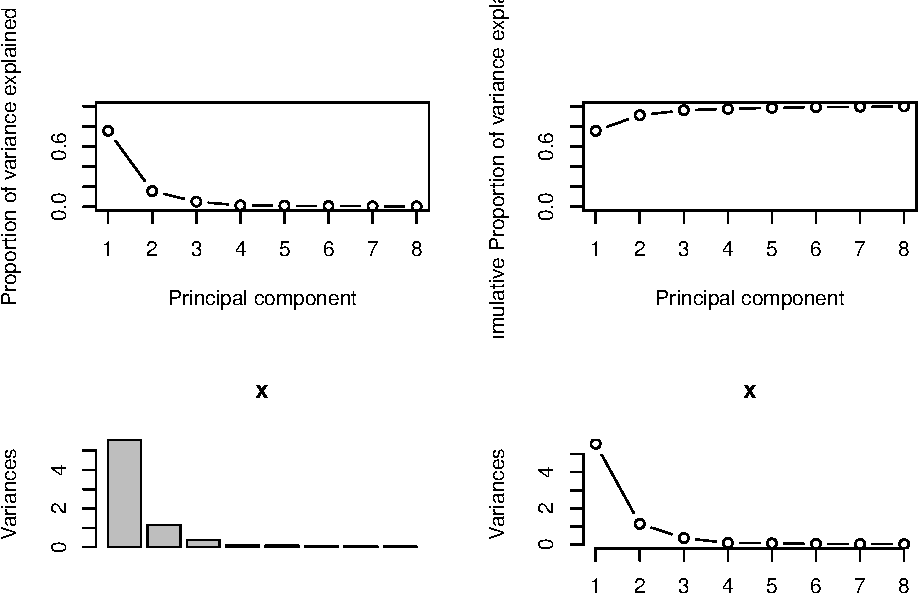
\includegraphics{Assignment_3_files/figure-latex/unnamed-chunk-7-1} \end{center}

\begin{itemize}
\item
  The top left skree plot, the proportion of variance explained
  decreased from the first principle component onward. This means the
  first principle component explains most of the variation in the
  dataset, second principle component explains the second most
  variation, and so on.
\item
  We can see that from the third principle component onward, the
  variance explained are minuscule. We can consider dropping them in
  favour of a lower dimension dataset since these principle components
  explain so little variance of the original dataset.
\item
  The bottom two graphs represent essentially the same information but
  measured in variance, which is also the eigen value of the covariance
  matrix of the original dataset.
\end{itemize}

\section{Principle Component Biplot}\label{principle-component-biplot}

\begin{Shaded}
\begin{Highlighting}[]
\NormalTok{g <-}\StringTok{ }\KeywordTok{ggbiplot}\NormalTok{(pc_car_pca, }\DataTypeTok{obs.scale =} \DecValTok{1}\NormalTok{, }\DataTypeTok{var.scale =} \DecValTok{1}\NormalTok{, }\DataTypeTok{labels=}\KeywordTok{row.names}\NormalTok{(pc_car),}
              \DataTypeTok{ellipse =} \OtherTok{TRUE}\NormalTok{, }
              \DataTypeTok{circle =} \OtherTok{TRUE}\NormalTok{)}
\NormalTok{g <-}\StringTok{ }\NormalTok{g }\OperatorTok{+}\StringTok{ }\KeywordTok{scale_color_discrete}\NormalTok{(}\DataTypeTok{name =} \StringTok{''}\NormalTok{)}
\NormalTok{g <-}\StringTok{ }\NormalTok{g }\OperatorTok{+}\StringTok{ }\KeywordTok{theme}\NormalTok{(}\DataTypeTok{legend.direction =} \StringTok{'horizontal'}\NormalTok{, }
               \DataTypeTok{legend.position =} \StringTok{'top'}\NormalTok{)}

\NormalTok{g <-}\StringTok{ }\NormalTok{g }\OperatorTok{+}\StringTok{ }\KeywordTok{labs}\NormalTok{(}\DataTypeTok{title =} \StringTok{"carm Principle Component Biplot"}\NormalTok{)}
\NormalTok{g}
\end{Highlighting}
\end{Shaded}

\begin{center}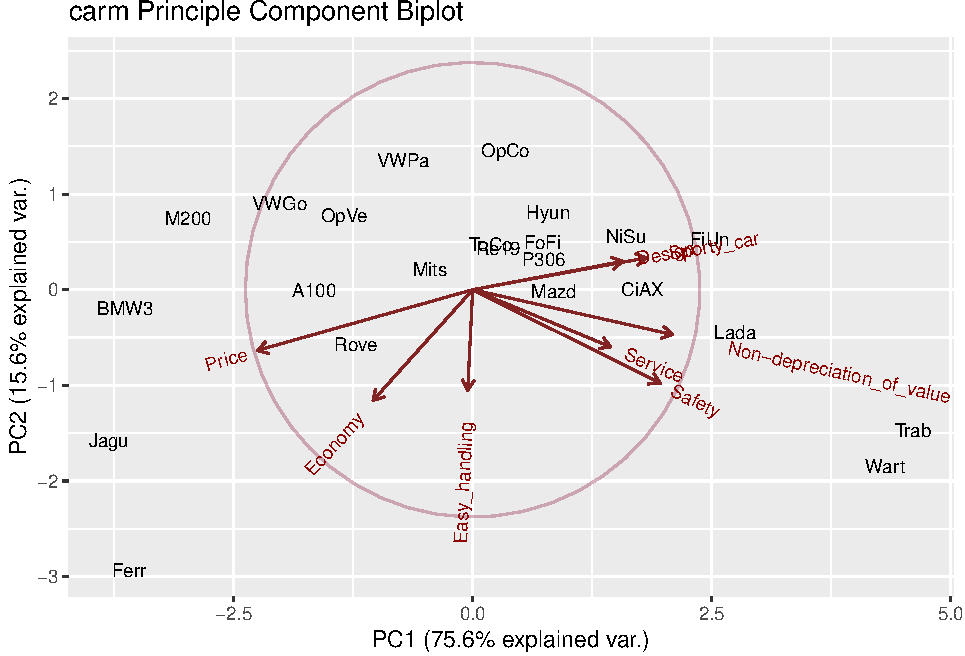
\includegraphics{Assignment_3_files/figure-latex/unnamed-chunk-8-1} \end{center}

\textbf{Interpretation of biplot} : For each car, the data set contains
scores on 8 different attributes: \texttt{Economy}, \texttt{Service},
\texttt{Non-depreciation\_of\_value}, \texttt{Price}, \texttt{Design},
\texttt{Sporty\_car}, \texttt{Safety}, and \texttt{Easy\_handling}. The
plot shows the first two Principal Component (PC) scores and the loading
vectors in a single biplot display.

\textbf{Interpreting car types} : The principal axes of this plot
represent PC1 and PC2 scores and individual cars are plotted on this
basis.

Cars that are close together have similar scores profiles. For example,
similar scores are given to \texttt{Trab} and \texttt{Wart} across all
eight attributes. This can also be interpreted as these two cars score
similarly across all eight attributes. The same is true for
\texttt{VWGo} and \texttt{OpVe}, although their scores are likely to be
very different then those about \texttt{Trab} and \texttt{Wart}, since
the two pairs of points are relatively far apart.

\textbf{Interpreting Loading Vectors} : The loading vectors are a
projected coordinate system for the original variables. So if a car is
projected perpendicularly onto, say, the \texttt{Price} vector - we
should get the relative \texttt{Price} score of that car. For example, a
\texttt{Jagu}, which has a \texttt{Price} score of 5.5, is very far
along in the direction of the \texttt{Price} vector; whereas a
\texttt{Trab} which has a \texttt{Price} score of 1.5 only, would be
very far along in the opposite direction of the \texttt{Price} vector if
we project it perpendicularly on to the \texttt{Price} vector.

A loading vector points in the direction which has the highest squared
multiple correlation with the Principal Components. Thus, \texttt{Price}
is better explained by PC1 than PC2 because its vector is pointing in
the direction closer to PC1; whereas \texttt{Easy\_handling} is much
better explained by PC2 because its vector overlaps almost entirely with
PC2. Vectors that point in the same direction correspond to attributes
that have similar weight on PC1 and/or PC2, and can be interpreted as
having the same meaning under the context of the dataset.

The length of the vector is proportional to the sum of the squared
correlation between the attribute and the PCs. The longer the vector,
the more correlated it is with PC1 and/or PC2. The \texttt{Price} vector
is almost touching the circumference of the unit circle, and thus well
explained by the first two PCs. On the other hand, the
\texttt{Easy\_handling} vector is much shorter, indicating that a large
portion of the variance is explained by the other PCs not drawn in this
plot.\\

\section{Correlation between the original variables and the first two
PCs.}\label{correlation-between-the-original-variables-and-the-first-two-pcs.}

\begin{Shaded}
\begin{Highlighting}[]
\NormalTok{n <-}\StringTok{ }\KeywordTok{nrow}\NormalTok{(pc_car)}
\NormalTok{sigma <-}\StringTok{ }\NormalTok{(n}\OperatorTok{-}\DecValTok{1}\NormalTok{) }\OperatorTok{*}\StringTok{ }\KeywordTok{cov}\NormalTok{(pc_car) }\OperatorTok{/}\StringTok{ }\NormalTok{n}
\NormalTok{CovYX <-}\StringTok{ }\KeywordTok{t}\NormalTok{(pc_car_pca}\OperatorTok{$}\NormalTok{rotation) }\OperatorTok\StringTok{ }\NormalTok{sigma}
\NormalTok{VarY<-}\StringTok{ }\KeywordTok{t}\NormalTok{(}\KeywordTok{eigen}\NormalTok{(sigma)}\OperatorTok{$}\NormalTok{vectors) }\OperatorTok\StringTok{ }\NormalTok{sigma }\OperatorTok\StringTok{ }\KeywordTok{eigen}\NormalTok{(sigma)}\OperatorTok{$}\NormalTok{vectors}
\NormalTok{DiagvarY<-}\StringTok{ }\KeywordTok{diag}\NormalTok{(}\DecValTok{1}\OperatorTok{/}\KeywordTok{sqrt}\NormalTok{(}\KeywordTok{diag}\NormalTok{(VarY)))}
\NormalTok{DiagSigma<-}\StringTok{ }\KeywordTok{diag}\NormalTok{(}\DecValTok{1}\OperatorTok{/}\KeywordTok{sqrt}\NormalTok{(}\KeywordTok{diag}\NormalTok{(sigma)))}
\NormalTok{CorYX <-}\StringTok{ }\NormalTok{DiagvarY }\OperatorTok\StringTok{ }\KeywordTok{t}\NormalTok{(pc_car_pca}\OperatorTok{$}\NormalTok{rotation) }\OperatorTok\StringTok{ }\NormalTok{sigma }\OperatorTok\StringTok{ }\NormalTok{DiagSigma}
\NormalTok{CorYX <-}\StringTok{ }\KeywordTok{t}\NormalTok{(CorYX)[,}\DecValTok{1}\OperatorTok{:}\DecValTok{2}\NormalTok{]}
\NormalTok{CorYX <-}\StringTok{ }\KeywordTok{cbind}\NormalTok{(CorYX, CorYX[,}\DecValTok{1}\NormalTok{]}\OperatorTok{^}\DecValTok{2} \OperatorTok{+}\StringTok{ }\NormalTok{CorYX[,}\DecValTok{2}\NormalTok{]}\OperatorTok{^}\DecValTok{2}\NormalTok{)}
\KeywordTok{colnames}\NormalTok{(CorYX) <-}\StringTok{ }\KeywordTok{c}\NormalTok{(}\KeywordTok{colnames}\NormalTok{(pc_car_pca}\OperatorTok{$}\NormalTok{rotation)[}\DecValTok{1}\OperatorTok{:}\DecValTok{2}\NormalTok{], }\StringTok{"r^2 sum"}\NormalTok{); }\KeywordTok{rownames}\NormalTok{(CorYX) <-}\StringTok{ }\KeywordTok{colnames}\NormalTok{(pc_car)}
\NormalTok{CorYX}
\end{Highlighting}
\end{Shaded}

\begin{verbatim}
##                                   PC1        PC2   r^2 sum
## Economy                   -0.60232608 -0.6698707 0.8115235
## Service                    0.89102745 -0.3690015 0.9300921
## Non-depreciation_of_value  0.96014130 -0.2154410 0.9682862
## Price                     -0.94756182 -0.2670751 0.9692025
## Design                     0.92302348  0.1747457 0.8825084
## Sporty_car                 0.88586934  0.1624741 0.8111623
## Safety                     0.87428086 -0.4354892 0.9540178
## Easy_handling             -0.04588907 -0.9331414 0.8728587
\end{verbatim}

This table confirms our findings in the biplot. In the leftmost two
columns, we can see that PC1 is indeed highly correlated to
\texttt{Price}, \texttt{Non-depreciation\_of\_value}, and
\texttt{Design}; PC2 is highly correlated to \texttt{Easy\_handling}
which correspond to the huge overlapping between the vector and the
axis.

The rightmost column shows the sum of squared correlation between the
first two PCs and each car attribute. This can be interpret as the
proportion of variance of the attribute explained by both PCs. Indeed,
\texttt{Price}, which has the largest \(r^{2}\) sum, also has the
longest loading vector.

\paragraph{For the sake of completeness, let's take a look at other
Principle
Components.}\label{for-the-sake-of-completeness-lets-take-a-look-at-other-principle-components.}

\begin{center}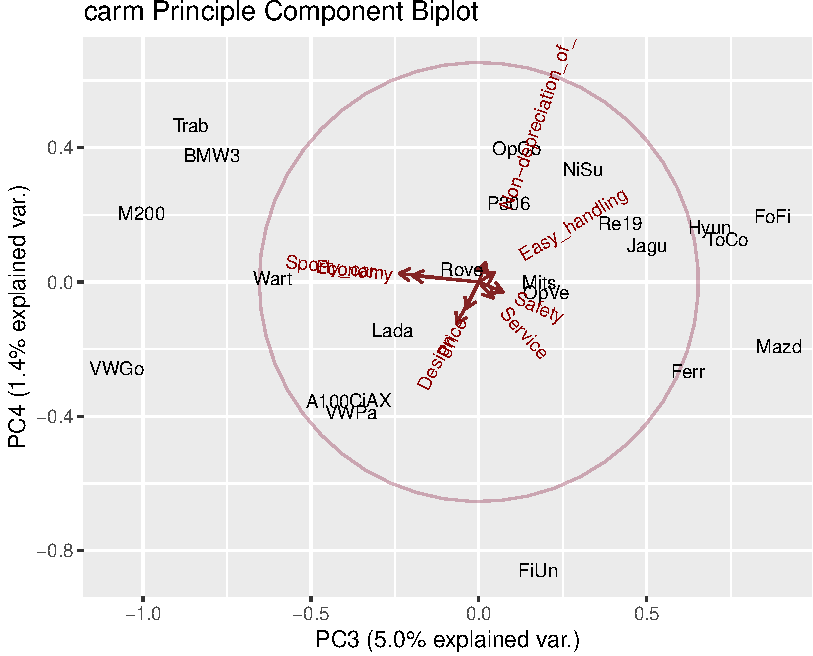
\includegraphics{Assignment_3_files/figure-latex/unnamed-chunk-10-1} \end{center}

This is the biplot of PC3 and PC4. Each vectors are very short because
the PCs in this plot explain so few of their variations. There are also
lots of overlapping between vectors, indicating the leftover variation
from PC1 and PC2 are mostly redundant.

\subsection{Summary on the cars (based on the first
biplot)}\label{summary-on-the-cars-based-on-the-first-biplot}

\begin{itemize}
\item
  The higher the car score on \texttt{Price} and \texttt{Economy} the
  lower it is scored on things like \texttt{Safety}, \texttt{Service},
  and \texttt{Non-depreciation\_of\_value}. So safety and services does
  come at a price. And it also makes sense that expensive cars are
  better at retaining values.
\item
  \texttt{Safety} and \texttt{Service} can be interpret as the same
  thing under context of the data, as their loading vector point in a
  very similar direction.
\item
  What you pay is what you get: the price tag directly reflect how good
  a car score on \texttt{Sporty\_car} and \texttt{Design}. The loading
  vector of \texttt{Price} and the other two are almost pointing at
  180\(^\circ\) away from each other. This means the higher the price,
  the better a car score at \texttt{Sporty\_car} and \texttt{Design}.
\item
  \texttt{Sporty\_car} and \texttt{Design} are essentially the same
  measure as their loading vectors overlap. Maybe people only appreciate
  the appearance of sporty cars these days.
\item
  Whether a car is a sports car has relatively little to do with the
  easiness to handle. The \texttt{Sporty\_car} loading vector points
  generally orthogonal (just a little more than 90\(^\circ\)) to the
  \texttt{Easy\_handling} vector.
\end{itemize}


\end{document}
